\begin{figure}[t]
\centering
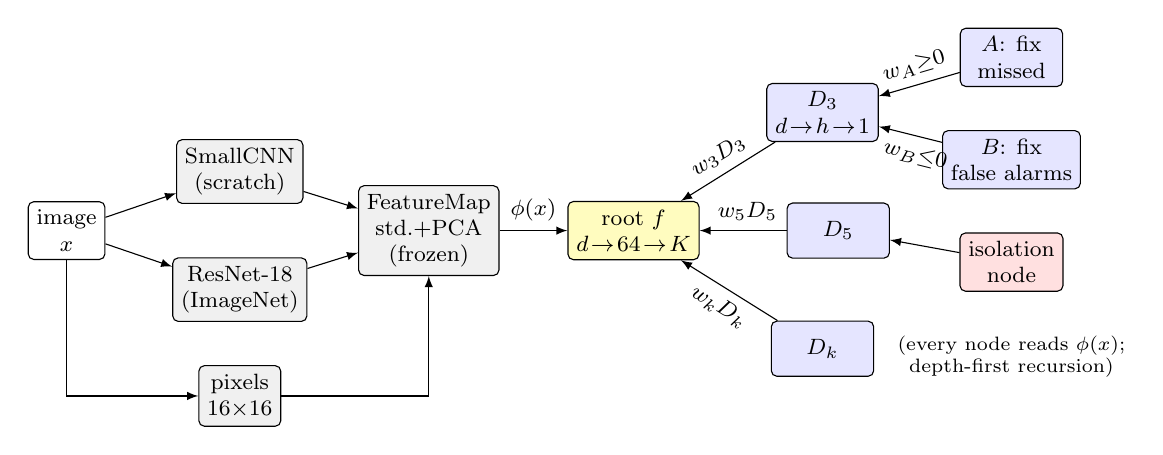
\begin{tikzpicture}[
  font=\footnotesize, >=latex,
  box/.style={draw, rounded corners=2pt, align=center, inner sep=3pt, minimum height=7mm},
  trunk/.style={box, fill=gray!12},
  node/.style={box, fill=blue!10, minimum width=13mm},
  root/.style={box, fill=yellow!25, minimum width=15mm},
  iso/.style={box, fill=red!12, minimum width=13mm},
]
\node[box, fill=white] (img) at (0,0) {image\\$x$};
\node[trunk] (t1) at (2.2,0.75) {SmallCNN\\(scratch)};
\node[trunk] (t2) at (2.2,-0.75) {ResNet-18\\(ImageNet)};
\node[trunk] (t0) at (2.2,-2.1) {pixels\\$16{\times}16$};
\node[trunk] (fm) at (4.6,0) {FeatureMap\\std.+PCA\\(frozen)};
\draw[->] (img) -- (t1); \draw[->] (img) -- (t2); \draw[->] (img) |- (t0);
\draw[->] (t1) -- (fm); \draw[->] (t2) -- (fm); \draw[->] (t0) -| (fm);
\node[root] (r) at (7.2,0) {root $f$\\$d\!\to\!64\!\to\!K$};
\draw[->] (fm) -- node[above]{$\phi(x)$} (r);
\node[node] (d1) at (9.6,1.5) {$D_3$\\$d\!\to\!h\!\to\!1$};
\node[node] (d2) at (9.8,0) {$D_5$};
\node[node] (d3) at (9.6,-1.5) {$D_k$};
\draw[->] (d1) -- node[above, sloped]{$w_3 D_3$} (r);
\draw[->] (d2) -- node[above, pos=0.45]{$w_5D_5$} (r);
\draw[->] (d3) -- node[below, sloped]{$w_k D_k$} (r);
\node[node] (a) at (12.0,2.2) {$A$: fix\\missed};
\node[node] (b) at (12.0,0.9) {$B$: fix\\false alarms};
\draw[->] (a) -- node[above, sloped]{$w_A{\ge}0$} (d1);
\draw[->] (b) -- node[below, sloped, pos=0.35]{$w_B{\le}0$} (d1);
\node[iso] (i1) at (12.0,-0.4) {isolation\\node};
\draw[->] (i1) -- (d2);
\node[font=\scriptsize, align=center] at (12.0,-1.6) {(every node reads $\phi(x)$;\\depth-first recursion)};
\end{tikzpicture}
\caption{Architecture. A frozen trunk and a frozen FeatureMap produce $\phi(x)$, which is shared by
every node. The $K$-way root is corrected by per-class detectors $D_k$ (our multiclass
generalisation of Table~II); every binary node is itself corrected by children $A$ (fires on its
misses) and $B$ (fires on its false alarms) exactly as in the note, recursively, with
closed-form isolation nodes as guaranteed-termination leaves. For Cats vs Dogs the root is a binary
node and the tree is the note's tree verbatim.}
\label{fig:arch}
\end{figure}
